\chapter{Implementation}\label{Implementation}

<this chapter outlines steps taken to simulate a working prototype of the design>
<this is used for evaluating the practical challenges faced by design>
<project work can be found online, as well as in appendix A>\footnote{https://github.com/tedski999/distributed-ech}

<look at how we simulate a deterministic, reproducible, configurable, measurable network environment with our own SSL certificates>
<how dns server can be configured to provide DoH with the designed publication strategy>
<tls server as well as configuration of standard ECH-enabled clients and web browsers>









\section{Simulation}

<simulation overview: qemu+bridge>

\subsection{Virtualisation}

<introduce qemu+debvm> \cite{bellard2005qemu}
<why problem: build is slow>
<build process, separating builder from hosts>
<using ssh to automate configuration>

\begin{listing}[ht]
\inputminted{bash}{snippets/build.bash}
\caption[Building OpenSSL from source inside build.img with DebVM]{TODO builder}
\end{listing}

<host base>
<boot up process>

\subsection{Networking}

<overview of networking and how it works with qemu>
<overview of linux networking devices>
<introduction to bridge networks>

\begin{listing}[ht]
\inputminted{bash}{snippets/br0.bash}
\caption[Connecting QEMU virtual machines using a network bridge]{TODO br0}
\end{listing}

<the static network configuration for simulation>
<using systemd to setup networking for all virtual machines at boot>

\begin{listing}[ht]
\inputminted{ini}{snippets/br0.ini}
\caption[Static bridge network configuration using systemd]{TODO /etc/systemd/network/00-br0.network contents}
\end{listing}

<introduction to openssl for certificates>
\cite{TODO:openssl}
<root certificate generated for simulation>

\begin{listing}[ht]
\inputminted{bash}{snippets/root.bash}
\caption[Generating a new self-signed root CA X.509 certificate using OpenSSL]{TODO root ca}
\end{listing}

<server certificates can be issued by the root ca as such>

\begin{listing}[ht]
\inputminted{bash}{snippets/dns.bash}
\caption[Signing a new X.509 certificate for ns.example.com using OpenSSL]{TODO dns}
\end{listing}

<with this we have a foundation for building networked virtual machines on top of>
<the rest of this chapter will be on how we implement these different types of servers and applications>










\section{DNS Server}

<one of the virtual machines operates as the dns server for the client to query>
<we use bind9 to provide this service>
\cite{TODO:bind}
<for practical ech client implementations that we will use, they require dns-over-https to use ech>
<we enable this using tls certificate as seen in fig>

\begin{listing}[ht]
\inputminted{bash}{snippets/bind}
\caption[DNS over HTTPS configuration using BIND 9]{TODO /etc/bind/named.conf contents}
\end{listing}

<bind9 uses zone files to specify>
<we will use them to specify all three dns designs>
<this first one is the simpler solution based on a records round robin but requiring a shared ech key>

\begin{listing}[ht]
\inputminted{zone}{snippets/shared.example.zone}
\caption[example.com zone file for distributed ECH using a shared ECH key]{}
\end{listing}

<as mentioned before, this is generally a security no no>
<we can do this>

\begin{listing}[ht]
\inputminted{zone}{snippets/separate.example.zone}
\caption[example.com zone file for distributed ECH using separate ECH keys]{}
\end{listing}

<this is a more involved, might break the spec and has shown mixed results>
<a dynamic dns service as such solves both of these issues>

\begin{listing}[ht]
\inputminted{zone}{snippets/dynamic.example.zone}
\caption[example.com zone file for distributed ECH using dynamic DNS]{}
\end{listing}

<this script will do this using nsupdate to send DNS zone updates>

\begin{listing}[ht]
\inputminted{zone}{snippets/dynamic.example.zone.bash}
\caption[Rudimentary script to implement a dynamic DNS service]{}
\end{listing}

<of course, this loses static configuration quality and is more complicated>











\section{TLS Server}

<remaining virtual machines operates as the co-operating tls servers>
<these servers are connected together over the bridge network>

<tls certs + ech key>

\begin{listing}[ht]
\inputminted{bash}{snippets/host_tls.bash}
\caption[Generating a new ECH key pair for tcd.example.com using OpenSSL]{TODO host+site tls}
\end{listing}

<use nginx as web server>
\cite{reese2008nginx}

\begin{listing}[ht]
\inputminted{nginx}{snippets/nginx}
\caption[Distributed ECH NGINX configuration for tcd.example.com]{TODO nginx}
\end{listing}

<wireguard vpn>\cite{donenfeld2017wireguard}

\begin{listing}[ht]
\inputminted{bash}{snippets/host_wg.bash}
\caption[Generating a new WireGuard key pair for tcd.example.com]{TODO host wg}
\end{listing}

<wireguard configuration>

\begin{listing}[ht]
\inputminted{ini}{snippets/host_wg.ini}
\caption[Configuring a WireGuard network interface using systemd]{TODO host wg}
\end{listing}

<wireguard peers>

\begin{listing}[ht]
\inputminted{ini}{snippets/host_wg0.ini}
\caption[Static WireGuard network configuration using systemd]{TODO host wg0}
\end{listing}

<use tc to pad traffic>
\cite{almesberger1999linux, hemminger2005network}

\begin{listing}[ht]
\inputminted{bash}{snippets/padding.bash}
\caption[Rudimentary script to shroud legitimate WireGuard communication]{}
\end{listing}

<all in all, works>











\section{TLS Client}

<recent work has been done to add ech support to many common clients>
<using several clients for qualitative and quantitative testing>
<for this project, we test with curl, firefox, chrome>
<we configure these clients to use our dns-over-https and ssl root>

\subsection{curl}

<introduction to curl>
<work by farrell>
<explanation of commands needed below>

\begin{listing}[ht]
\inputminted{nginx}{snippets/curl.bash}
\caption[Command to use ECH-enabled curl on QEMU virtual machines]{TODO curl}
\end{listing}

<challenges>
<working>

\subsection{Mozilla Firefox}

<introduction to firefox>
<explanation of config needed for below>

\begin{figure}[ht]
\centerline{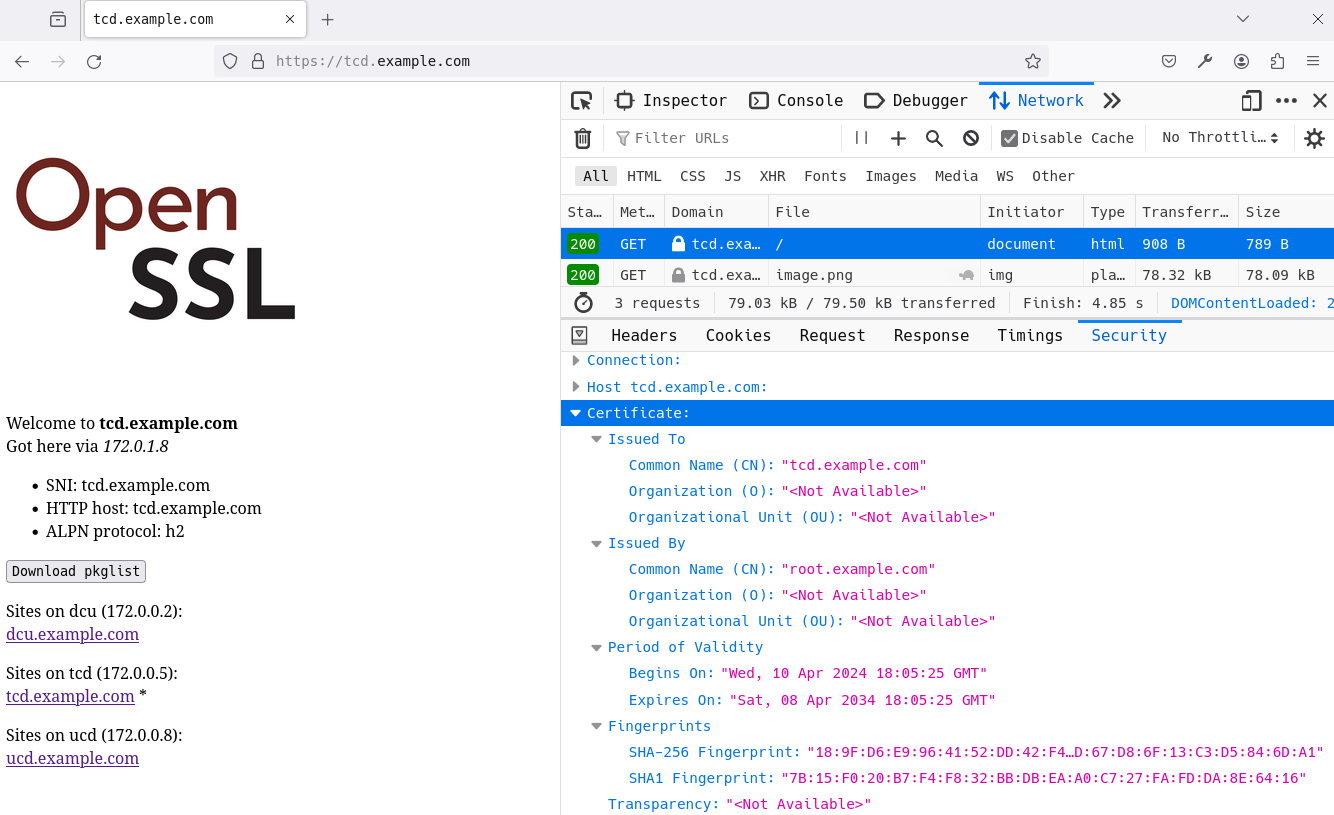
\includegraphics[width=120mm]{images/firefox.png}}
\caption[Screenshot of Mozilla Firefox when accessing tcd.example.com]{<TODO>}
\label{firefox_screenshot_figure}
\end{figure}

<challenges>
<working>

\subsection{Google Chrome}

<introduction to chrome>
<explanation of config needed for below>

\begin{figure}[ht]
\centerline{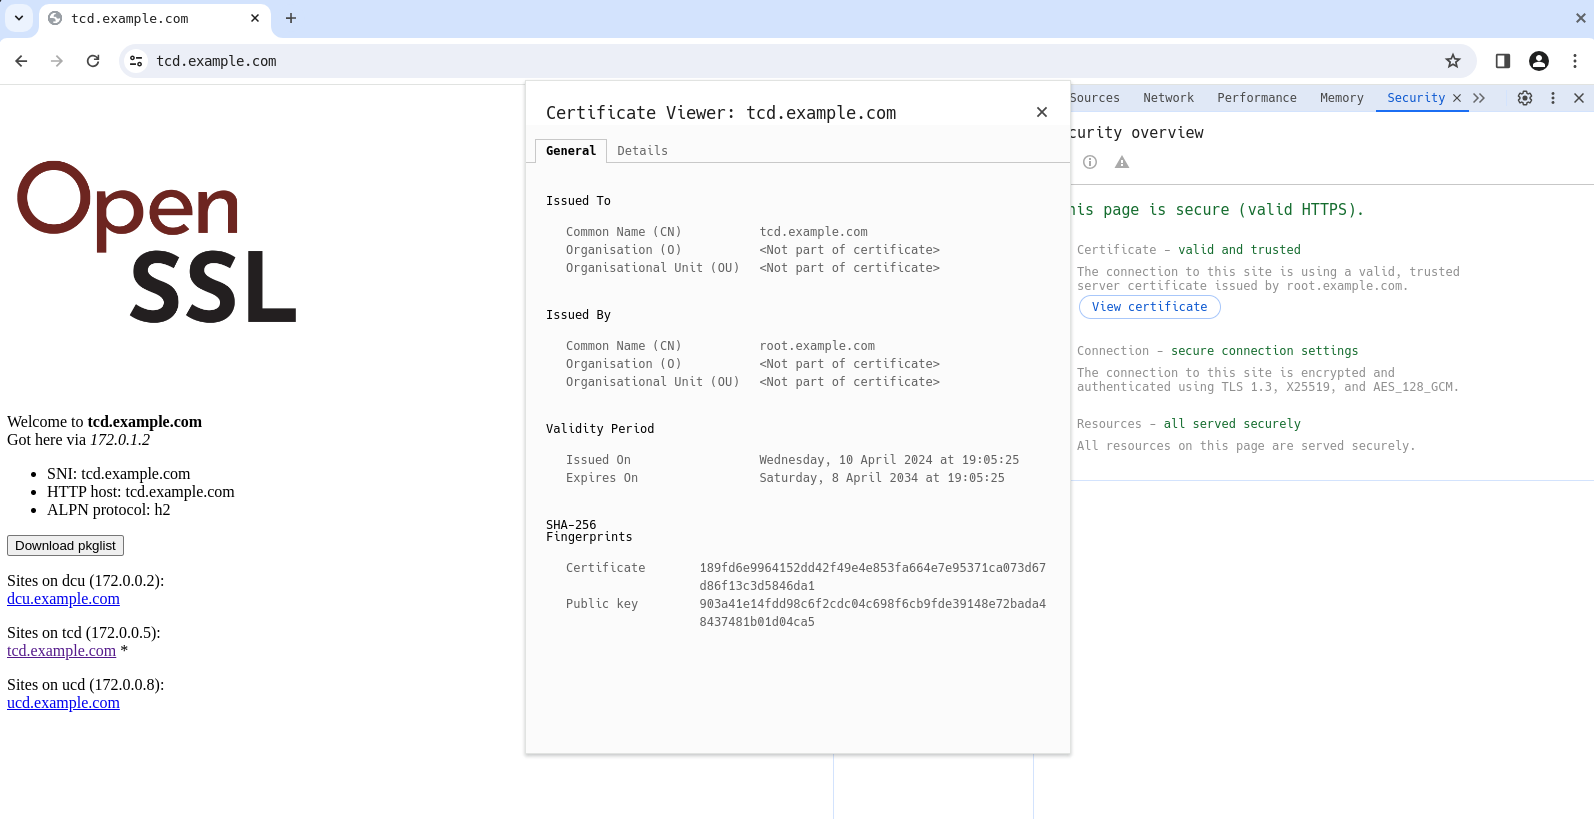
\includegraphics[width=120mm]{images/chrome.png}}
\caption[Screenshot of Google Chrome when accessing tcd.example.com]{<TODO>}
\label{chrome_screenshot_figure}
\end{figure}

<challenges>
<working>











\section{Summary}

<this chapter has presented an implementation of the design for testing purposes>
<simulated using qemu with debvm>
<bind9 is used for dns>
<nginx is used as web server>
<wireguard and tc for traffic obfuscation>
<curl, firefox and chrome as clients>
